\documentclass[12pt, a4paper, twoside]{report}
\usepackage[utf8]{inputenc}
\usepackage[T1,T2A]{fontenc}

\usepackage[russian, english]{babel}
\usepackage{xcolor} %for transparency
\usepackage{graphicx}

\usepackage{indentfirst}

\newcommand{\HRule}{\rule{\linewidth}{0.5mm}}
%\setcounter{section}{1}
\renewcommand{\thesection}{\arabic{section}}

%Rename contents - magic here
\addto\captionsenglish{% Replace "english" with the language you use
	  \renewcommand{\contentsname}%
	      {Оглавление}%
      }
%END rename contents

\begin{document}

\begin{titlepage}
\begin{center}
\fontencoding{T1}\selectfont

\textsc{\LARGE Liceum Boarding School number 2}\\[1.5cm]

\textsc{\Large Some crappy project}\\[0.5cm]

% Title
\HRule \\[0.4cm]
{ \huge \bfseries Tesseract and hyperplane investigation\\[0.4cm] }

\HRule \\[1.5cm]

% Author and supervisor
\noindent
\begin{minipage}{0.4\textwidth}
\begin{flushleft} \large
\emph{Authors:}\\
Ilgic \textsc{Mustafin} \newline
\fontencoding{T2A}\selectfont
Гриша \textsc{Maxxx} \newline %USE RUSSIAN FONT
\fontencoding{T1}\selectfont %USE LATIN HERE
Mirolin \textsc{M} 
and \newline
Arthur \textsc{Nugmanov} 
\end{flushleft}
\end{minipage}%
\begin{minipage}{0.4\textwidth}
\begin{flushright} \large
\emph{Supervisor:} \\
Marsel \textsc{Abiy}
\end{flushright}
\end{minipage}

\vfill

% Bottom of the page
{\large \today}

\end{center}
\end{titlepage}
 %Load titlepage so we do not mess up the numeration

\tableofcontents

\newpage
\section{Введение}
Введение, тезисы, примерное описание работы.
Данная работа ставит своей целью создать математическую модель пересечения четырехмерного гиперкуба или тессеракта трехмерной гиперплоскость, а также создать программную имплементацию данной математической задачи. Предполагается рассмотреть варианты возможных сечений данного гиперкуба.

Как известно, гиперкуб представляет собой куб в четырехмером пространстве, может также называться тетракубом и тессерактом. В даннной работе будет рассматриваться представление данной фигуры в виде множества точек в Евклидовом пространстве $(\pm 1,\pm 1,\pm 1, \pm 1)$. Тессеракт ограничивают 8 гиперплоскостей, т.е.подпространств, на единицу меньшей чем объемлющее пространство.


\section{Тессеракт, или четырехмерный гиперкуб}
\begin{figure}[h!]
	\center
	\framebox{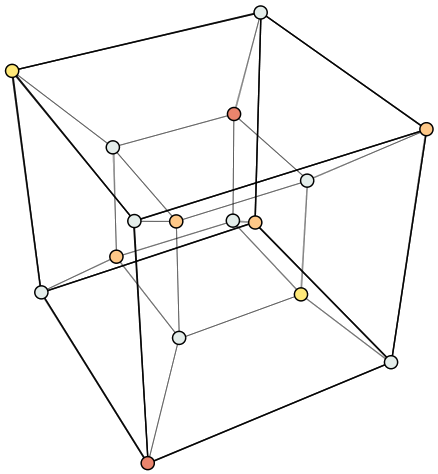
\includegraphics[scale=0.5]{./tesseract_fig1.png}}
	\clearpage
\end{figure}
Описание 4 пространства. Описать аналогию и методы перехода 3-4D в аналитической геометрии.
\section{Мат. аппарат}

\section{Описание работы программы}
\section{Примеры сечений}
\subsection{Тетраэдр}

\subsection{Пятигранная призма}
\subsection{Шестигранная призма}
0 1 0 1
1 0 1 1
0 1 1 1
0 0 0 0
\section{Тессеракт в культуре}
\subsection{В литература}
\subsection{В кинематографе}
\subsection{В мифологии(прим. жидорептилоиды)}
\section{Заключение}
\section{Список используемой литературы}
\section{Приложения}

\end{document}

